\mathchardef\mhyphen="2D
\documentclass[11pt]{article}
\usepackage[english]{babel}
\usepackage{minted}
\usepackage{amsfonts}
\usepackage{amsmath}
\usepackage{amsthm}
\usepackage{amssymb}
\usepackage{graphicx}
\usepackage{subcaption}
\usepackage[hypcap=false]{caption}
\usepackage{booktabs}
\usepackage[left=25mm, top=25mm, bottom=25mm, right=25mm]{geometry}
\usepackage{soul}
\usepackage{algorithm}
\usepackage{algpseudocode}
\usepackage[most]{tcolorbox}
\usepackage[colorlinks=true,linkcolor=darkcyan,filecolor=darkcerulean,urlcolor=magenta]{hyperref}
\usepackage{braket}
\usepackage{quantikz}
\usepackage{svg}

\newcommand{\calA}{\mathcal{A}}
\newcommand{\calB}{\mathcal{B}}
\newcommand{\calC}{\mathcal{C}}
\newcommand{\calD}{\mathcal{D}}
\newcommand{\calE}{\mathcal{E}}
\newcommand{\calF}{\mathcal{F}}
\newcommand{\calG}{\mathcal{G}}
\newcommand{\calH}{\mathcal{H}}
\newcommand{\calI}{\mathcal{I}}
\newcommand{\calJ}{\mathcal{J}}
\newcommand{\calK}{\mathcal{K}}
\newcommand{\calL}{\mathcal{L}}
\newcommand{\calM}{\mathcal{M}}
\newcommand{\calN}{\mathcal{N}}
\newcommand{\calO}{\mathcal{O}}
\newcommand{\calP}{\mathcal{P}}
\newcommand{\calQ}{\mathcal{Q}}
\newcommand{\calR}{\mathcal{R}}
\newcommand{\calS}{\mathcal{S}}
\newcommand{\calT}{\mathcal{T}}
\newcommand{\calU}{\mathcal{U}}
\newcommand{\calV}{\mathcal{V}}
\newcommand{\calW}{\mathcal{W}}
\newcommand{\calX}{\mathcal{X}}
\newcommand{\calY}{\mathcal{Y}}
\newcommand{\calZ}{\mathcal{Z}}

\newcommand{\bfA}{\mathbf{A}}
\newcommand{\bfB}{\mathbf{B}}
\newcommand{\bfC}{\mathbf{C}}
\newcommand{\bfD}{\mathbf{D}}
\newcommand{\bfE}{\mathbf{E}}
\newcommand{\bfI}{\mathbf{I}}
\newcommand{\bfS}{\mathbf{S}}
\newcommand{\bfP}{\mathbf{P}}
\newcommand{\bfQ}{\mathbf{Q}}
\newcommand{\bfU}{\mathbf{U}}
\newcommand{\bfv}{\mathbf{v}}
\newcommand{\bfu}{\mathbf{u}}
\newcommand{\bfdelta}{\mathbf{\Delta}}
\newcommand{\bfpi}{\mathbf{\Pi}}


\newcommand{\N}{\mathbb{N}}
\newcommand{\z}{\mathbb{Z}}
\newcommand{\I}{\mathbb{I}}
\newcommand{\C}{\mathbb{C}}

\newcommand{\keygen}{\mathsf{KeyGen}}
\newcommand{\enc}{\mathsf{Enc}}
\newcommand{\dec}{\mathsf{Dec}}
\newcommand{\negl}{\mathsf{negl}}
\newcommand{\commit}{\mathsf{Commit}}
\newcommand{\ccommit}{\mathsf{C\text{-}Commit}}

\newcommand{\setup}{\mathsf{Setup}}
\newcommand{\lsetup}{\mathsf{Setup\text{-}Lossy}}

\newcommand{\samplemat}{\mathsf{Sample\text{-}Dirac\text{-}Matrix}}
\newcommand{\eval}{\mathsf{Eval}}
\newcommand{\obf}{\mathsf{Obf}}

\newcommand{\phybb}[1]{p_{\mathrm{hyb}, #1}}
\newcommand{\lin}{\ell_{\mathrm{in}}}
\newcommand{\lout}{\ell_{\mathrm{out}}}
\newcommand{\bit}{\{0,1\}}
\newcommand{\sd}{\mathsf{SD}}
\newcommand{\lwe}{\mathsf{LWE}_{n,m,q,\chi}}
\newcommand{\sslwe}[4]{\mathsf{ss\text{-}LWE}_{#1,#2,#3,#4}}
\newcommand{\sslwec}{\sslwe{n}{m}{q}{\chi}}

\newcommand{\unif}[1]{\mathsf{Unif}_{\left[-#1, #1\right]}}
\newcommand{\func}[2]{\mathsf{Func}[#1, #2]}
\newcommand{\perm}[2]{\mathsf{Perm}[#1, #2]}
\newcommand{\ct}{\mathsf{ct}}
\newcommand{\Finverse}{F^{-1}}

\newcommand{\nqss}{\mathsf{No\mhyphen Query \mhyphen Semantic \mhyphen Security}}

\newcommand{\Tr}{\mathrm{Tr}}
\newcommand{\trace}[1]{\Tr\left( #1 \right)}

\newcommand{\prob}[1]{\Pr\left[ #1 \right]}

\newcommand{\brakett}[2]{\braket{#1|#2}}
\newcommand{\ketbraa}[2]{\ket{#1}\bra{#2}}
\newcommand{\ketbra}[1]{\ketbraa{#1}{#1}}

\newcommand{\lddh}{\mathcal{L}_{DDH}}
\newcommand{\lnddh}{\mathcal{L}_{nDDH}}
\newcommand{\lddhkt}{\mathcal{L}_{DDH,k,t}}

\newlength{\protowidth}
\newcommand{\pprotocol}[4]{
{\begin{center}
\setlength{\protowidth}{\textwidth}
\addtolength{\protowidth}{-3\intextsep}

\fbox{
        \small
        \hbox{\quad
        \begin{minipage}{\protowidth}
    \begin{center}
    {\bf #1}
    \end{center}
        #4
        \end{minipage}
        \quad}
        }
        \captionof{figure}{\label{#3} #2}
\end{center}
} }

\newcommand{\defbox}[1]{
{\begin{center}
\setlength{\protowidth}{\textwidth}
\addtolength{\protowidth}{-3\intextsep}

\fcolorbox{darkcerulean}{cottoncandy}{
        \small
        \hbox{\quad
        \begin{minipage}{\protowidth}
    
        #1
        \end{minipage}
        \quad}
        }
\end{center}
        } }

\newcommand{\protocol}[4]{
\pprotocol{#1}{#2}{#3}{#4} }

\newtheorem{theorem}{Theorem}[section]
\newtheorem{claim}[theorem]{Claim}
\newtheorem{fact}[theorem]{Fact}
\newtheorem{definition}[theorem]{Definition}
\newtheorem*{question}{Question}

\newtcolorbox[auto counter,number within=section]{solution}[1][]{every float=\centering,breakable,enhanced,adjusted title={Question \thetcbcounter},#1,colback=codegray,colframe=darkcerulean!50!black}

\linespread{1.0}

\definecolor{codegray}{rgb}{0.98,0.97,0.93}
\definecolor{cottoncandy}{rgb}{1.0, 0.84, 0.95}
\definecolor{darkcerulean}{rgb}{0.03, 0.27, 0.49}
\definecolor{darkcyan}{rgb}{0.0, 0.50, 0.45}

\title{C S 358H: Intro to Quantum Information Science}
\author{Sayam Sethi}
\date{October 2024}

\begin{document}

\maketitle

\tableofcontents

\pagenumbering{arabic}

\newpage

\section{Kinda-dense coding}
We said in class that superdense quantum coding requires 1 ebit of
entanglement between Alice and Bob, in addition to 1 qubit of
communication.  In this problem, however, we'll see how to do a ``poor
man's" dense quantum coding with no entanglement, just 1 qubit of
communication from Alice to Bob.

Suppose Alice knows two bits, $x$ and $y$.  She'd like to let Bob learn either bit of his choice, $x$ or
$y$, though not necessarily both of them (and she doesn't know which Bob
is interested in).
\begin{solution}[label=ques:1]
  \begin{question}
    Work out an explicit circuit of Toffoli gates for adding two 2-bit integers to get a 3-bit integer --- assume the integers are unsigned, encoded in binary in the usual, simplest way. You can use arbitrary ancilla bits initialized to 0 or 1. Be sure to designate your input, output, and garbage registers. 

\noindent Show the garbage bits that are generated by your circuit when 11 is added to 10.
  \end{question}
  \tcblower{}
  \begin{proof}
    The circuit that performs a full-adder for a 2-bit unsigned addition is:

    \begin{minipage}{\textwidth}
      \begin{quantikz}
        \lstick{$a_0$} & \ctrl{5} & \ctrl{6} & \slice{} &          &          & \slice{} &          & \slice{} & \\
        \lstick{$a_1$} &          &          &          & \ctrl{7} & \ctrl{6} &          &          &          & \\
        \lstick{$b_0$} & \ctrl{3} &          & \ctrl{4} &          &          &          &          &          & \\
        \lstick{$b_1$} &          &          &          & \ctrl{5} &          & \ctrl{4} &          &          & \\
        \lstick{$1$}   &          & \ctrl{2} & \ctrl{2} &          & \ctrl{3} & \ctrl{3} &          & \ctrl{3} & \\
        \lstick{$c_0$} & \targ{}  &          &          &          &          &          & \ctrl{3} & \ctrl{2} & \\
        \lstick{$s_0$} &          & \targ{}  & \targ{}  &          &          &          &          &          & \\
        \lstick{$s_1$} &          &          &          &          & \targ{}  & \targ{}  & \ctrl{1} & \targ{}  & \\
        \lstick{$s_2$} &          &          &          & \targ{}  &          &          & \targ{}  &          & 
      \end{quantikz}
    \end{minipage}

    We represent the two 2-bit inputs as $a_1a_0$ and $b_1b_0$ and the output as $s_2s_1s_0$. The circuit uses 8 Toffoli gates.\par
    To see why it works, note that the group of three Toffolis before the first slice, and the group of three Toffolis between the first and second slice perform the same function but on different input and output bits. The first Toffoli in the sequence computes the carry bit ($c_0, s_2$) and the next two Toffolis compute the xor of the input bits to get the sum ($s_0, s_2$). The two Toffolis before the last slice are used to incorporate the carry bit from the first addition into the sum bits $s_1, s_2$. We use two garbage bits $1, c_0$, for executing CNOTs and storing the carry, respectively.\par
    When $11$ is added to $10$, we have $a_1a_0 = 11$ and $b_1b_0 = 10$. The output of the circuit is $s_2s_1s_0 = 101$ and the garbage bits are $c_0 = 0$ and $1 = 1$.
  \end{proof}
\end{solution}


\newpage

\section{Non-local operations}
\begin{solution}[label=ques:2a]
  \begin{question}
    Calculate $QFT_2, QFT_3,$ and $QFT_4$ explicitly (either by writing down the corresponding matrix or equivalently by specifying the action on each of the standard basis states).  By what other name
is $QFT_2$ known?
  \end{question}
  \tcblower{}
  \begin{proof}[Solution]
    We have,
    \begin{equation}
      \begin{split}
        QFT_2 &= \frac{1}{\sqrt{2}}\begin{pmatrix}
          1 & 1 \\
          1 & -1
        \end{pmatrix}\text{, also known as the Hadamard gate} \\
        QFT_3 &= \frac{1}{\sqrt{3}}\begin{pmatrix}
          1 & 1 & 1 \\
          1 & \omega & \omega^2 \\
          1 & \omega^2 & \omega
          \end{pmatrix}\text{, where }\omega = e^{2\pi/3} \\
        QFT_4 &= \frac{1}{2}\begin{pmatrix}
          1 & 1 & 1 & 1 \\
          1 & i & -1 & -i \\
          1 & -1 & 1 & -1 \\
          1 & -i & -1 & i
          \end{pmatrix}
      \end{split}
      \label{eq:qft_comp}
    \end{equation}
  \end{proof}
\end{solution}

\begin{solution}[label=ques:2b]
  \begin{question}
    Prove that $QFT_d$ is unitary for all $d$.
  \end{question}
  \tcblower{}
  \begin{proof}
    We will show that $QFT_d$ is a unitary by showing that $\brakett{QFT_d\ket{x_1}}{QFT_d\ket{x_2}} = 0$ for any orthonormal basis vector $x_1 \neq x_2$ and it is equal to $1$ when $x_1 = x_2$ (this is equivalent to showing that the columns of $QFT_d$ form an orthonormal basis):
    \begin{equation}
      \begin{split}
        \brakett{QFT_d\ket{x_1}}{QFT_d\ket{x_2}} &= \brakett{\frac{1}{\sqrt{d}}\sum^{d-1}_{y=0}\omega^{x_1y}\ket{y}}{\frac{1}{\sqrt{d}}\sum^{d-1}_{z=0}\omega^{x_2z}\ket{z}}\\
        &= \frac{1}{\sqrt{d}}\sum_{y=0}^{d-1}\sum_{z=0}^{d-1}\omega^{-x_1y}\omega^{x_2z}\brakett{y}{z}\\
        &= \frac{1}{\sqrt{d}}\sum_{y=0}^{d-1}(\omega^{-x_1})^y(\omega^{x_2})^y = \frac{1}{\sqrt{d}}\sum_{y=0}^{d-1}(\omega^{x_2-x_1})^y\\
        &= \begin{cases}
          1, &\text{ if }x_1 = x_2\\
          0, &\text{ otherwise}
        \end{cases}
      \end{split}
      \label{eq:qft_unitary}
    \end{equation}
    Hence, proved that $QFT_d$ is unitary for all $d$.
  \end{proof}
\end{solution}

\begin{solution}[label=ques:2c]
  \begin{question}
    For which values of $d$ is $QFT_d$ its own inverse?
  \end{question}
  \tcblower{}
  \begin{proof}[Solution]
    $QFT_d$ is its own inverse when $QFT_d = QFT_d^\dagger$. We have,
    \begin{equation}
      \begin{split}
        &(QFT_d)_{ij} = (QFT_d^\dagger)_{ij}\\
        \implies &\frac{1}{\sqrt{d}}\omega^{ij} = \frac{1}{\sqrt{d}}\omega^{-ij}\\
        \implies &\omega^{2ij} = 1\\
        \implies &e^{4\pi ij/d} = 1\text{ for all }i, j \in \{0,1,...,d-1\}\\
        \implies &d = 1, 2
      \end{split}
      \label{eq:qft_inverse}
    \end{equation}
    Therefore, $QFT_d$ is its own inverse for $d = 1, 2$.
  \end{proof}
\end{solution}

\begin{solution}[label=ques:2d]
  \begin{question}
    In Recitation 4, we saw that the qudit clock and shift matrices are respectively defined as $X_d\ket{x} = \ket{x + 1 \bmod d}$ and $Z_d\ket{x} = \omega^x\ket{x}$ for $x \in 0,1,\ldots,d-1$. Show that $$QFT_d^\dagger X_d QFT_d = Z_d^\dagger.$$
  \end{question}
  \tcblower{}
  \begin{proof}
    We will show this relation holds by showing it holds for every basis state $x \in \{0, 1, \ldots, d-1\}$:
    \begin{equation}
      \begin{split}
        QFT_d^\dagger X_d QFT_d\ket{x} &= QFT_d^\dagger X_d\left(\frac{1}{\sqrt{d}}\sum_{y=0}^{d-1}\omega^{xy}\ket{y}\right)\\
        &= QFT_d^\dagger\left(\frac{1}{\sqrt{d}}\sum_{y=0}^{d-1}\omega^{xy}\ket{y+1 \bmod d}\right)\\
        &= QFT_d^\dagger\left(\frac{1}{\sqrt{d}}\sum_{y=0}^{d-1}\omega^{x(y+1)}\omega^{-x}\ket{y+1 \bmod d}\right)\\
        &= \omega^{-x}QFT_d^\dagger\left(\frac{1}{\sqrt{d}}\sum_{y=0}^{d-1}\omega^{x(y+1 \bmod d)}\ket{y+1 \bmod d}\right)\\
        &= \omega^{-x}QFT_d^\dagger\left(\frac{1}{\sqrt{d}}\sum_{z=0}^{d-1}\omega^{xz}\ket{z}\right)\\
        &= \omega^{-x}QFT_d^\dagger\left(QFT_d\ket{x}\right)\\
        &= \omega^{-x}\ket{x}\\
        &= Z_d^\dagger\ket{x}
      \end{split}
      \label{eq:qft_xz}
    \end{equation}
    Since Equation~\ref{eq:qft_xz} is true for all basis states, we have $QFT_d^\dagger X_d QFT_d = Z_d^\dagger$.
  \end{proof}
\end{solution}


\newpage

\section{The GHZ Game}
In the ``GHZ game'', there are three players, Alice, Bob, and
Charlie, who are given bits $x$, $y$, and $z$ respectively.  We're promised
that $x+y+z=0 \pmod{2}$; otherwise the bits can be arbitrary.  The
players' goal is, without communicating with each other, to output
bits a, b, c respectively such that
$a+b+c = \text{OR}(x,y,z) \pmod{2}$.
In other words, they should collectively output an odd number of 1-bits if and
only if at least one of the input bits is 1.

\begin{solution}[label=ques:3]
  \begin{question}
    Give two different decompositions of the 1-qubit mixed state $$\rho = \begin{bmatrix}\cos^2(\pi/8) & 0\\ 0 & \sin^2(\pi/8)\end{bmatrix}$$ as a mixture of two pure states. Show your work. What do these decompositions correspond to physically?
Draw a 2D-sketch of the Bloch sphere to aid your explanation.
  \end{question}
  \tcblower{}
  \begin{proof}[Solution]
    One trivial decomposition for the given state $\rho$ is $\cos^2\pi/8$ probability of having the $\ket{0}$ state and $\sin^2\pi/8$ probability of measuring the $\ket{1}$ state.\par
    Now, for obtaining a second possible decomposition, we compute the coefficients of $\rho$ in the generalised representation of any state in the Bloch sphere. We have
    \begin{equation}
      \begin{split}
        &\rho = \frac{1}{2}\left(\bfI + x\bfX + y\bfY + z\bfZ\right)\\
        \implies &\cos^\pi/8 = 1 + z, \sin^2\pi/8 = 1 - z, x + iy = 0, x - iy = 0\\
        \implies &z = 2\cos^2\pi/8 - 1 = \cos\pi/4 = \frac{1}{\sqrt{2}}, x = y = 0
      \end{split}
      \label{eq:blochdecomp}
    \end{equation}
    Therefore, the state $\rho$ is on the $Z$ axis with the $z$ coordinate of $\frac{1}{\sqrt{2}}$. Now, let us try to decompose the state with one state as the $\ket{+}$ state (this has coordinates $(1, 0, 0)$). Now, let us assume that the other state $\ket{\psi}$ will have coordinates $(x, y, z)$. We can write $\rho$ in terms of density matrices given by $\ket{+}$ and $\ket{\psi}$ as
    \begin{equation}
      \begin{split}
        &\rho = p\ketbra{+} + (1 - p)\ketbra{\psi}\text{, where $p$ is the probability of the $\ket{+}$ state}\\
        \implies &\left(0, 0, \frac{1}{\sqrt{2}}\right) = p(1, 0, 0) + (1 - p)(x, y, z)\\
        \implies &0 = p + (1 - p)x, 0 = (1 - p)y, \frac{1}{\sqrt{2}} = (1 - p)z\\
        \implies &x = \frac{p}{p - 1}, y = 0, z = \frac{1}{\sqrt{2}(1 - p)}\text{ ($y = 0$ since $p = 1$ gives a contradiction)}
      \end{split}
      \label{eq:rhodecomp}
    \end{equation}
    Now, we also know that $x^2 + y^2 + z^2 = 1$ since $\ket{\psi}$ is a pure state and therefore, we can solve for $p$ and we get $p = \frac{1}{4}$. Now, we can compute $x$ and $z$ as
    \begin{equation}
      x = \frac{-1}{3}, z = \frac{2\sqrt{2}}{3}
      \label{eq:xzsol}
    \end{equation}
    Therefore, we can write $\ket{\psi}$ as
    \begin{equation}
      \ket{\psi} = \frac{2\sqrt{2} - 1}{3}\ket{0} - \frac{1}{3}\ket{1}
      \label{eq:psisol}
    \end{equation}
    Therefore, we have another decomposition for $\rho$ as $\ket{+}$ with probability $\frac{1}{4}$ and $\ket{\psi}$ with probability $\frac{3}{4}$.
    We show the different decompositions in the Bloch sphere below

    \centerline{\begin{minipage}[t]{\textwidth}
      \centering
      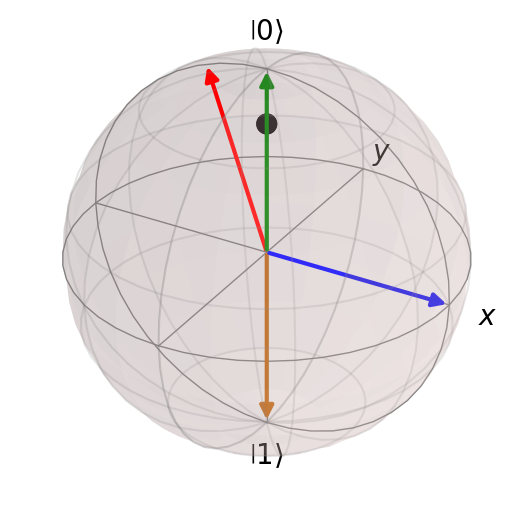
\includegraphics[width=0.5\textwidth]{bloch_sphere.png}
      \captionof{figure}{Bloch sphere indicating the different decompositions. The black circle indicates the position of $\rho$. The states in green and yellow are the states $\ket{0}$ and $\ket{1}$ respectively. The states in blue and red are the states $\ket{+}$ and $\ket{\psi}$ respectively. The lines connecting each of these pairs of states passes through $\rho$.}\label{fig:bloch}
    \end{minipage}}
  \end{proof}
\end{solution}


\newpage

\section{Noisy CHSH}
Suppose Alice and Bob share a Bell pair $\frac{1}{\sqrt{2}}(\ket{00}+\ket{11})$. Imagine that unbeknownst to Alice and Bob, their qubits are not completely isolated from the outside world: with probability $\epsilon$, one of the qubits is measured in the $\{\ket{0},\ket{1}\}$ basis by the ``environment'' and the state of their pair collapses to either the state $\ket{00}$ or $\ket{11}$ (with probability $1-\epsilon$, the qubits remain in the Bell state).\par
\textit{Recall:} In the CHSH game, Alice and Bob receive independent random bits $x$ and $y$ respectively. Their goal is to output bits $a$ and $b$ respectively such that $a+b=xy \pmod{2}$. No communication is allowed.  In the ``usual strategy'', Alice does nothing to her qubit if $x=0$ and she applies a $\frac{\pi}{4}$ counterclockwise rotation towards $\ket{1}$ if $x=1$. Bob applies a $\frac{\pi}{8}$ counterclockwise rotation if $y=0$ and he applies a $\frac{\pi}{8}$ \textit{clockwise} rotation, toward $-\ket{1}$ if $y=1$. Alice and Bob both measure their qubits in the $\{ \ket{0},\ket{1} \}$ basis and output whatever they see. This strategy wins $\cos^2\left(\frac{\pi}{8}\right) \approx 85\%$ of the time, while any classical strategy can win with probability at most $3/4$.

\begin{solution}{Part a}\label{ques:4a}
  \begin{question}
    But what if $\ket{\psi}$ is either $\ket{0}$ or $\ket{+}$ (with equal probability)? Give the protocol that distinguishes the two states with with a failure probability of $\sin^2(\frac{\pi}{8})\approx .146$. Show explicitly that your protocol achieves this failure probability.
\\ Note that when we ask for a protocol, we mean some step-by-step algorithm that ends by outputting ``I think this was $\ket{0}$'' or ``I think this was $\ket{+}$''.
\\ Hint: Read Section 5.2 of the textbook.
  \end{question}
  \tcblower{}
  \begin{proof}
    We propose the following protocol,
    \protocol{Protocol to distinguish between $\ket{0}$ and $\ket{+}$}{Distinguishing protocol}{proto:diff}{
      \begin{enumerate}
        \item Apply the $R_X(\pi/8)$ gate to the input state $\ket{\psi}$ (i.e., rotate the state by $\pi/8$ along the $X$ axis).
        \item Measure the state in the standard basis.
        \item If the measurement result is $\ket{0}$, output $\ket{0}$, else output $\ket{+}$.
      \end{enumerate}
    }
    We now prove that the failure probability of this protocol is $\sin^2(\pi/8)$. If we had the $\ket{0}$ state, then the state of the qubit after applying the rotation gate is $\cos\frac{\pi}{8}\ket{0} + \sin\frac{\pi}{8}\ket{1}$. Alternatively, if we started with the $\ket{+}$ state, the state would be $\cos\frac{3\pi}{8}\ket{0} + \sin\frac{3\pi}{8}\ket{1}$. Now, the failure probability can be computed as,
    \begin{equation}
      \begin{split}
        \prob{\text{failure}} &= \frac{1}{2}\cdot\prob{\text{failure }| \ket{\psi} = \ket{0}} + \frac{1}{2}\cdot\prob{\text{failure }| \ket{\psi} = \ket{+}}\\
        &= \frac{1}{2}\cdot\sin^2\frac{\pi}{8} + \frac{1}{2}\cdot\cos^2\frac{3\pi}{8}\\
        &= \frac{1}{2}\cdot\sin^2\frac{\pi}{8} + \frac{1}{2}\cdot\sin^2\frac{\pi}{8} = \sin^2\frac{\pi}{8}
      \end{split}
    \end{equation}
    Hence, we have shown that the failure probability of this protocol is $\sin^2(\pi/8)$.
  \end{proof}
\end{solution}

\begin{solution}{Part b}\label{ques:4b}
  \begin{question}
    Prove that this is optimal.
  \end{question}
  \tcblower{}
  \begin{proof}
    Any protocol that will be used to distinguish the two states can be represented as a unitary on some $n$ qubits, followed by measurements in the standard basis at the end. Any intermediate measurements can be deferred to the end by adding more qubits in the circuit (for each intermediate measurement, add an extra qubit, perform a CNOT between the qubit to be measured and the new qubit and instead measure the new qubit; now this new qubit isn't involved in any further operations so its measurement can be done at any point, we do it at the end along with all other measurements).\par
    Therefore, any protocol has the effect of performing a measurement in a certain orthonormal basis. However, we know that no unitary can change the inner product between two states. This implies that the angle between the two states is still fixed at $\theta = \cos^{-1}\left|\brakett{\psi_1}{\psi_2}\right|$. Thus, the most optimal basis to measure the two states will have each orthonormal state at an angle of some $\alpha$ and $\alpha + \theta$ from the two states (assuming that $\theta$ is acute, the argument is similar for an obtuse $\theta$). Therefore the least failure probability for any protocol is $2\cdot \frac{1}{2}\cdot \cos^2\alpha = \cos^2(\pi/2 - \theta/2) = \sin^2\theta/2$.\par
    For the states $\ket{0}$ and $\ket{+}$, the angle is $\pi/4$ and therefore the best failure probability is $\sin^2\pi/8$.
  \end{proof}
\end{solution}

\begin{solution}{Part c}\label{ques:4c}
  \begin{question}
    What is the failure probability if you measure in the $\{\ket{0}, \ket{1}\}$ basis?
  \end{question}
  \tcblower{}
  \begin{proof}[Solution]
    If we measure in the $\{\ket{0}, \ket{1}\}$ basis and guess that the state was $\ket{+}$ only if the measurement result is $\ket{1}$, the failure probability can be computed as,
    \begin{equation}
      \begin{split}
        \prob{\text{failure}} &= \frac{1}{2}\cdot\prob{\text{failure }| \ket{\psi} = \ket{0}} + \frac{1}{2}\cdot\prob{\text{failure }| \ket{\psi} = \ket{+}}\\
        &= 0 + \frac{1}{2}\cdot\frac{1}{2}\text{, since there is a 50\% probability of getting }\ket{1}\\
        &= \frac{1}{4}
      \end{split}
    \end{equation}
  \end{proof}
\end{solution}


\end{document}
